\documentclass[conference,onecolumn]{IEEEtran} % or twocolumn
\usepackage{cite}
\usepackage[pdftex]{graphicx}
%\usepackage[cmex10]{amsmath}
%\usepackage{algorithmic}
%\usepackage[tight,footnotesize]{subfigure}
%\usepackage[font=footnotesize]{subfig}
%\usepackage{url}

% correct bad hyphenation here
\hyphenation{op-tical net-works semi-conduc-tor}

\begin{document}
%
% paper title
% can use linebreaks \\ within to get better formatting as desired
\title{CE481 Team2 Term Project Proposal}


% author names and affiliations
% use a multiple column layout for up to three different
% affiliations
\author{
\IEEEauthorblockN{Duckyu Choi}
\IEEEauthorblockA{Dept. Civil and Environmental Engineering\\ KAIST}
}


% make the title area
\maketitle


\begin{abstract}
%\boldmath
The abstract goes here. The abstract goes here. The abstract goes here. The abstract goes here.
The abstract goes here. The abstract goes here. The abstract goes here. The abstract goes here.
The abstract goes here. The abstract goes here. The abstract goes here. The abstract goes here.
\end{abstract}


\section{Introduction}
% no \IEEEPARstart
Introduction goes here. Introduction goes here. Introduction goes here. Introduction goes here.
Introduction goes here. Introduction goes here. Introduction goes here. Introduction goes here.
Introduction goes here. Introduction goes here. Introduction goes here. Introduction goes here.

\subsection{Subsection Heading Here}
Subsection text here. Subsection text here. Subsection text here. Subsection text here.


\subsubsection{Subsubsection Heading Here}
Subsubsection text here. Subsubsection text here. Subsubsection text here. Subsubsection text here.

\begin{figure}[!h]
  \centering
    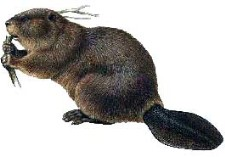
\includegraphics[width=2.5in]{beaver.jpg}
  \caption{Simulation Results}
  \label{figlabel}
\end{figure}

As can be seen in Fig. \ref{figlabel}, example figure can be placed as below.
Subsubsection text here. Subsubsection text here. Subsubsection text here. Subsubsection text here.

\begin{table}[!h]
% increase table row spacing, adjust to taste
\renewcommand{\arraystretch}{1.3}
  \caption{An Example of a Table}
  \label{tablelabel}
  \centering
  \begin{tabular}{|c||c|}
  \hline
  One & Two\\
  \hline
  Three & Four\\
  \hline
  \end{tabular}
\end{table}

As can be seen in \ref{tablelabel}, example table can be placed as below. Subsubsection text here. Subsubsection text here. Subsubsection text here. Subsubsection text here.

\section{Conclusion}
The conclusion goes here. The conclusion goes here. The conclusion goes here. The conclusion goes here This is how to cite a paper \cite{jung2018multi}. Look at references.bib file for more details.

% use section* not to add number in the front
\section*{Acknowledgment}
The authors would like to thank...


% references section
\IEEEtriggeratref{5}
\bibliographystyle{IEEEtran}
\bibliography{references}


% that's all folks
\end{document}


